\documentclass{article}
\usepackage[utf8]{inputenc}
\usepackage{graphicx}

\begin{document}
\title{Exercise 2 of the Computer Vision course at the
  University of Helsinki in May 2018}

\author{\emph{Konsta Kutvonen}}
\maketitle


\newpage
\section{Hands on exercises}

\subsection{Strawberry modifications}

I found that running dilate and then close, I was able to quite well remove the holes in the strawberries and the pixels disappeared with just an erosion, or better yet with just an open that also didn't remove that much of the strawberries. I wasn't able to find a good combination that would have allowed for both of these to take place in my experimentations.

\fbox{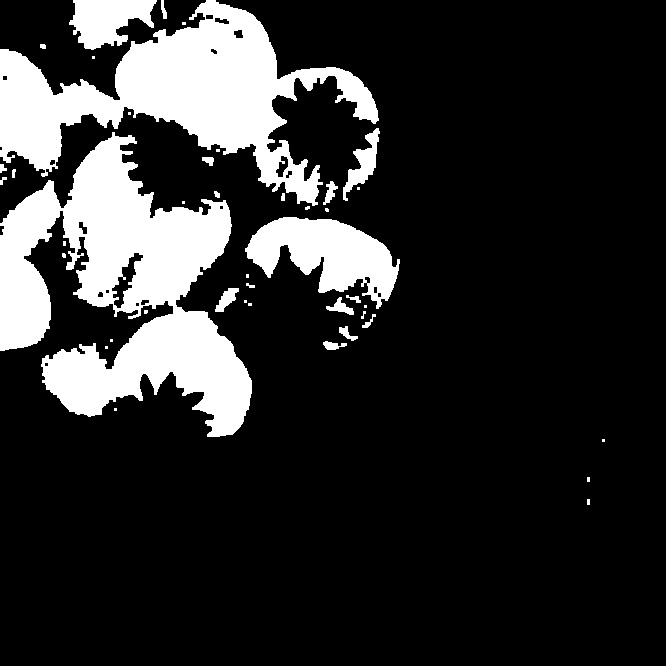
\includegraphics[height=70mm]{closedstrawberry}}
\fbox{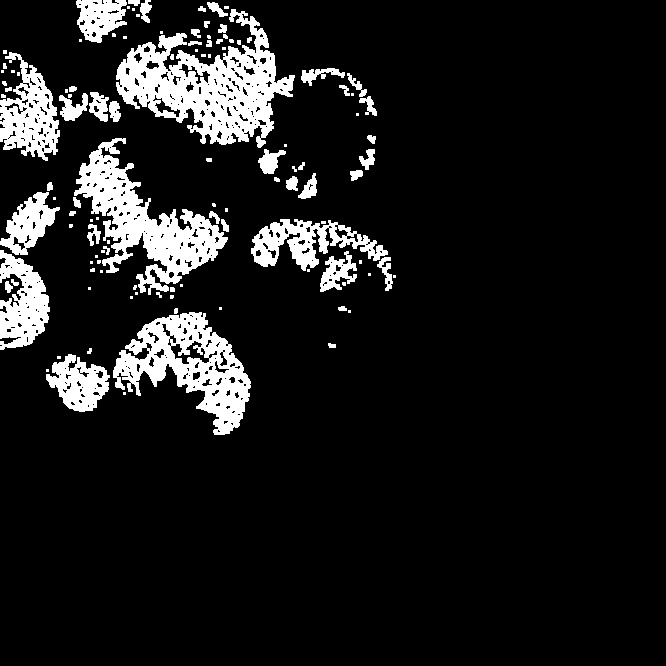
\includegraphics[height=70mm]{nopixelstrawberry}}
\newpage
\subsection{Transforming the house}
Here is the blurred house. I used blur intensities 51, 101, 151, 201 and 301.
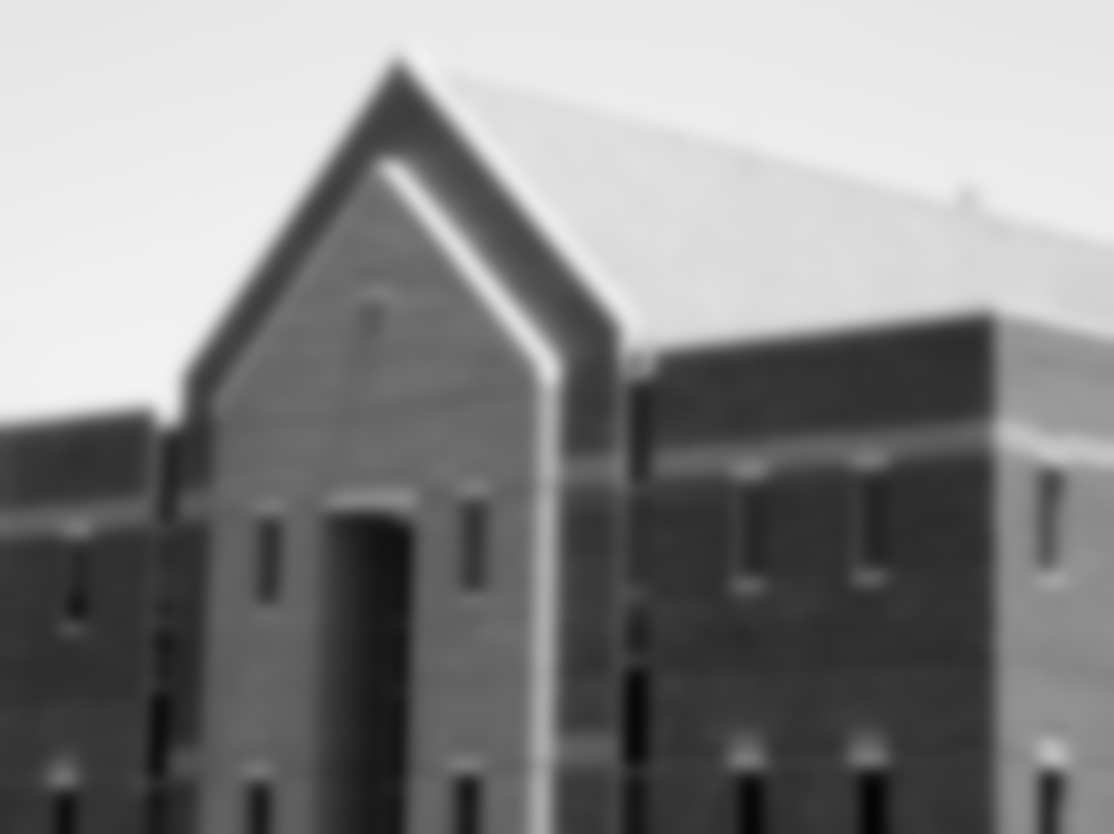
\includegraphics[height=60mm]{blurredhouse51}
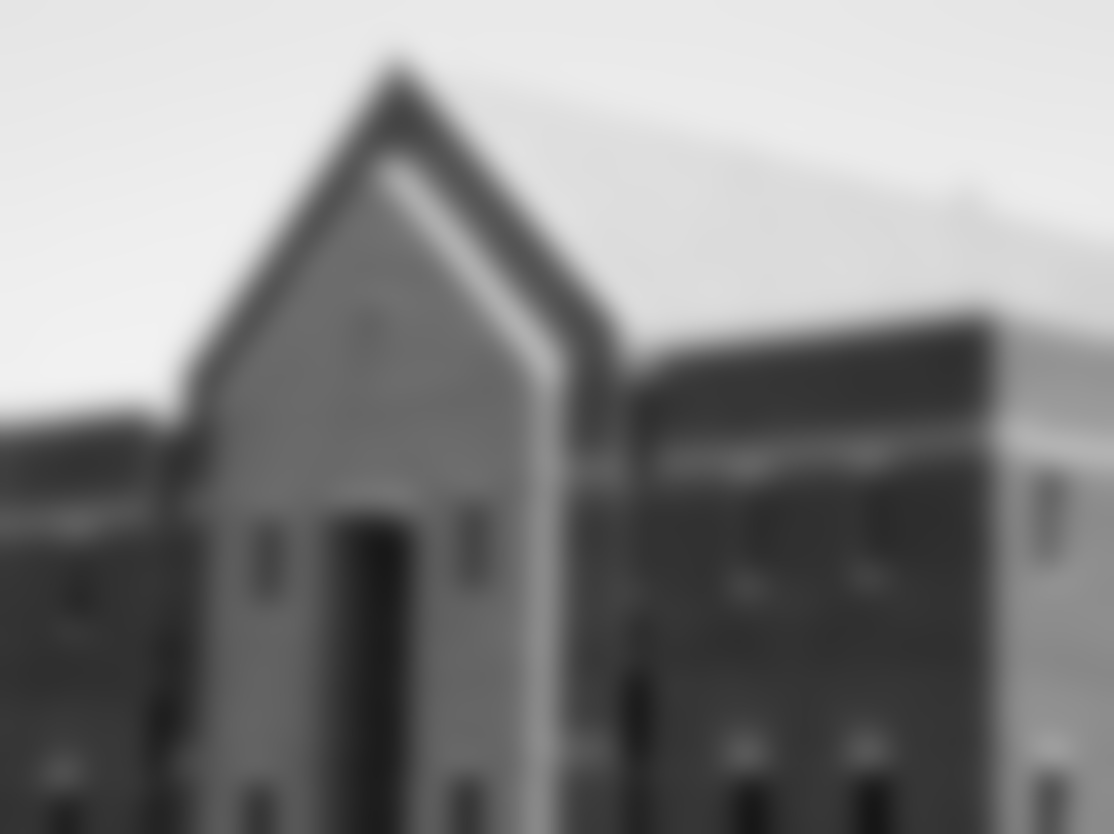
\includegraphics[height=60mm]{blurredhouse101}
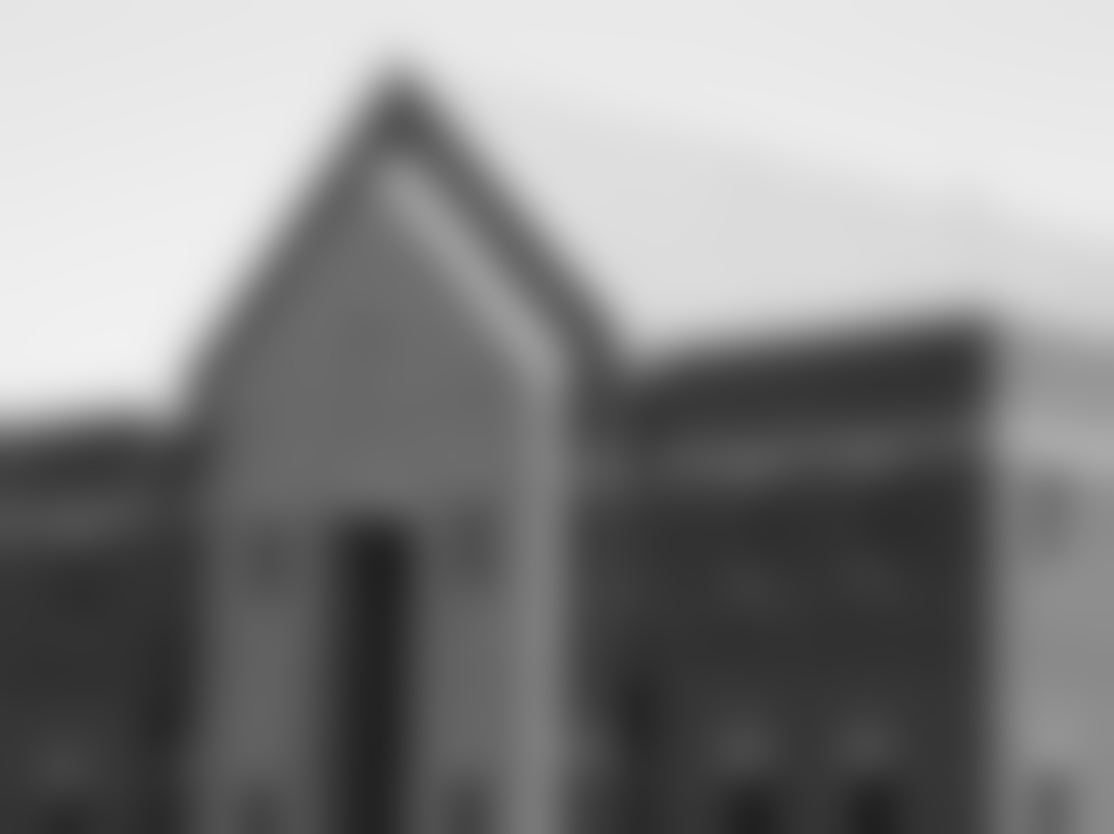
\includegraphics[height=60mm]{blurredhouse151}
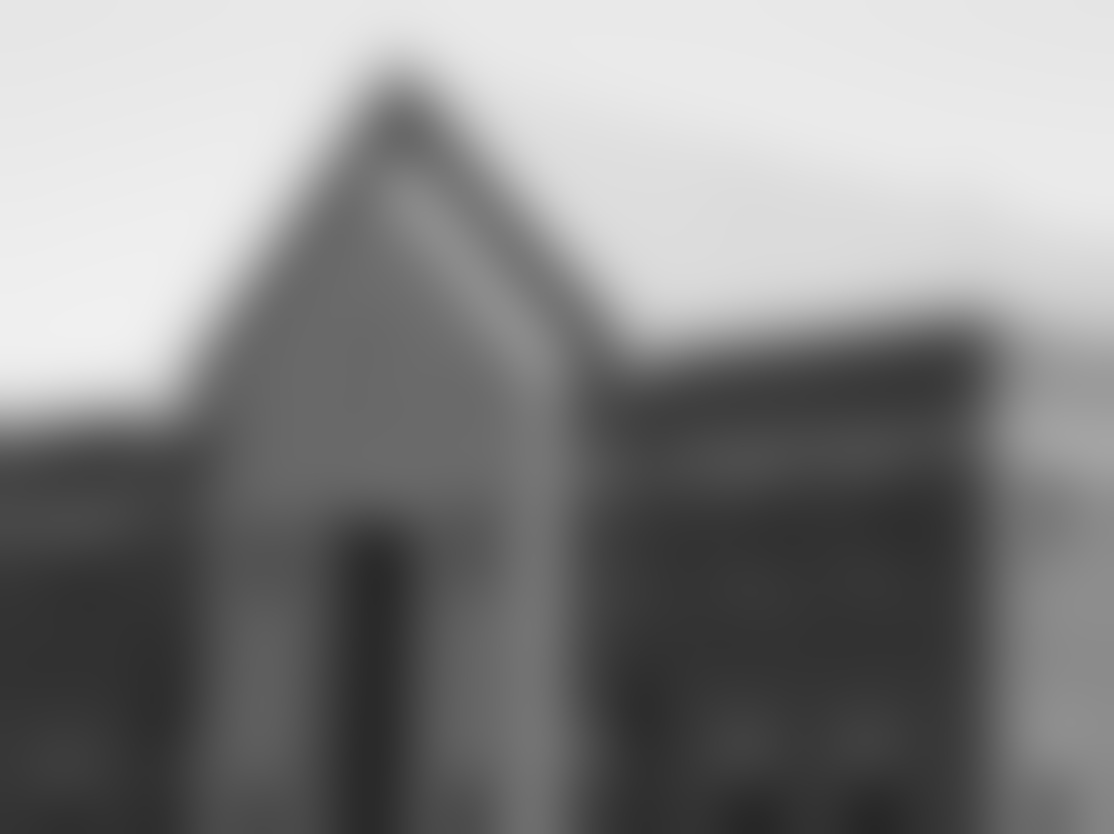
\includegraphics[height=60mm]{blurredhouse201}
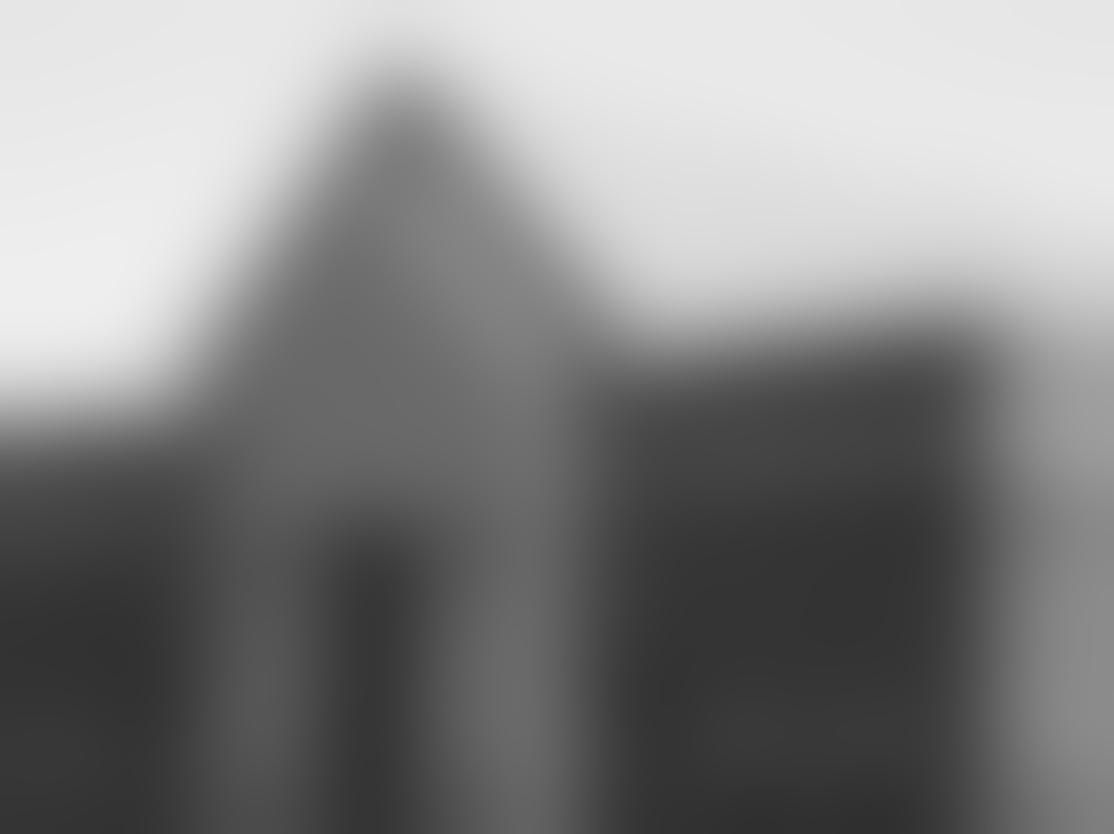
\includegraphics[height=60mm]{blurredhouse301}
\newpage

Here is laplace house
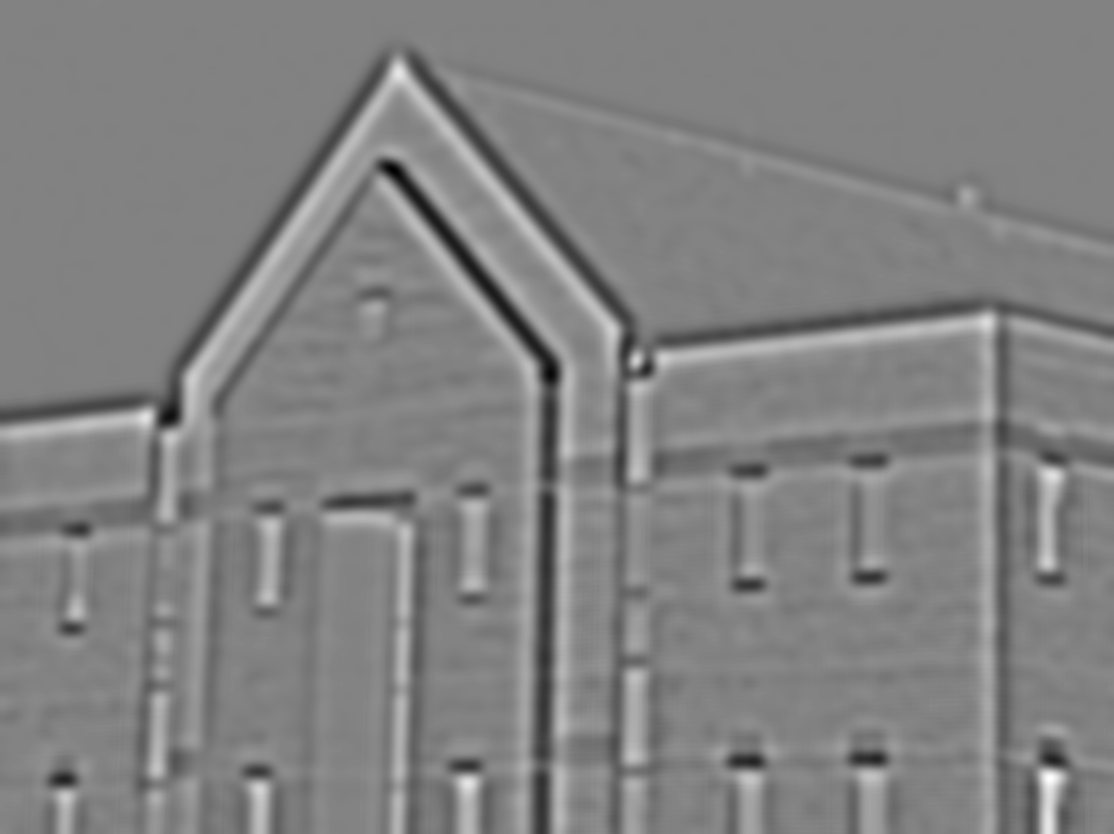
\includegraphics[height=60mm]{laplace51}
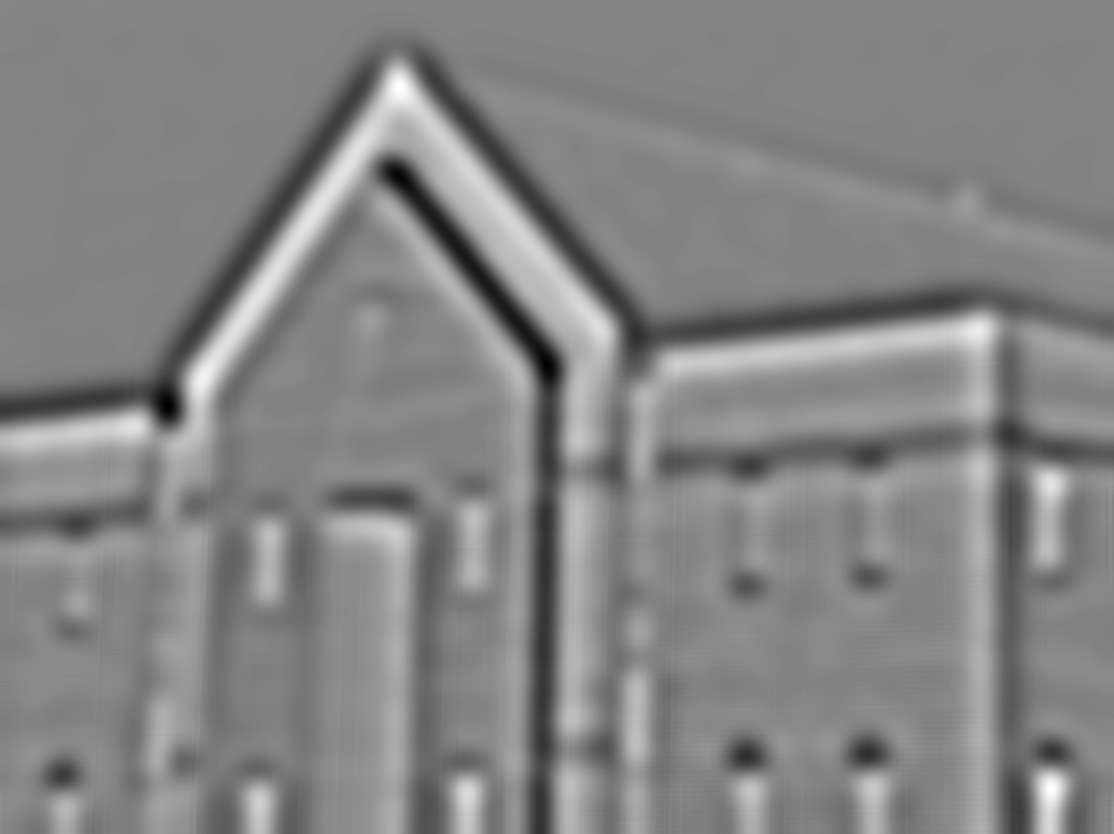
\includegraphics[height=60mm]{laplace101}
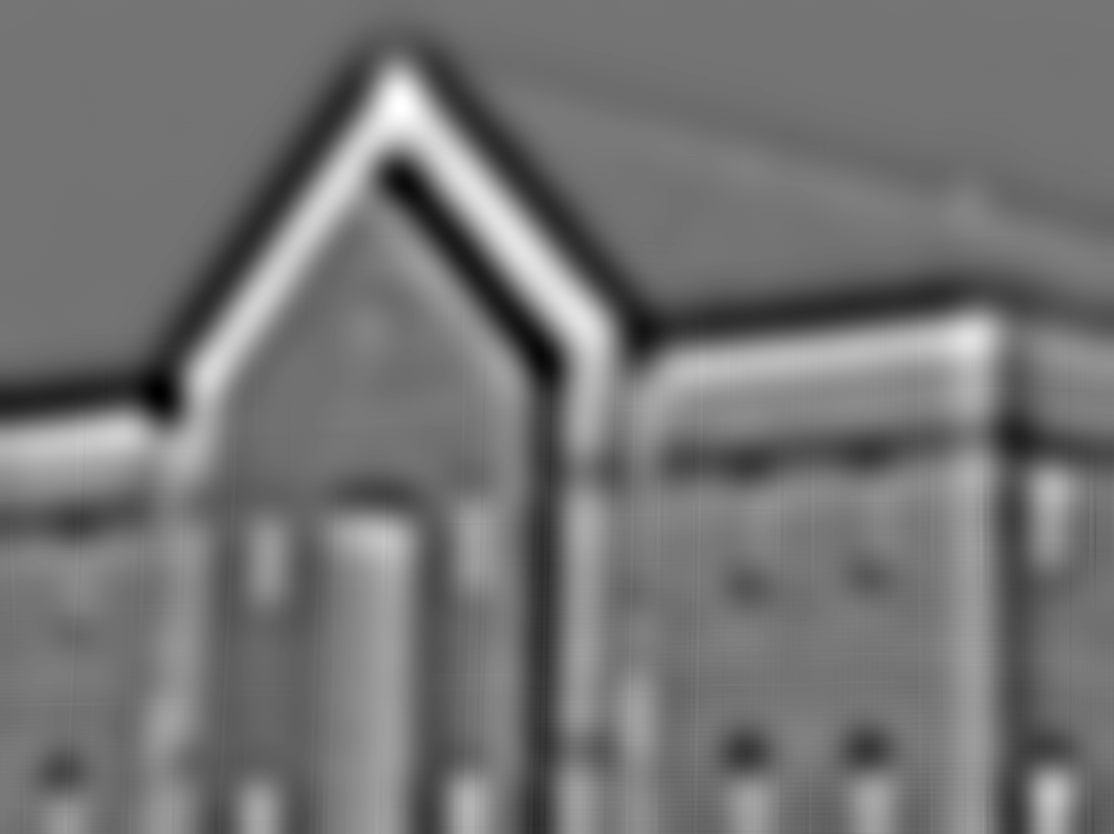
\includegraphics[height=60mm]{laplace151}
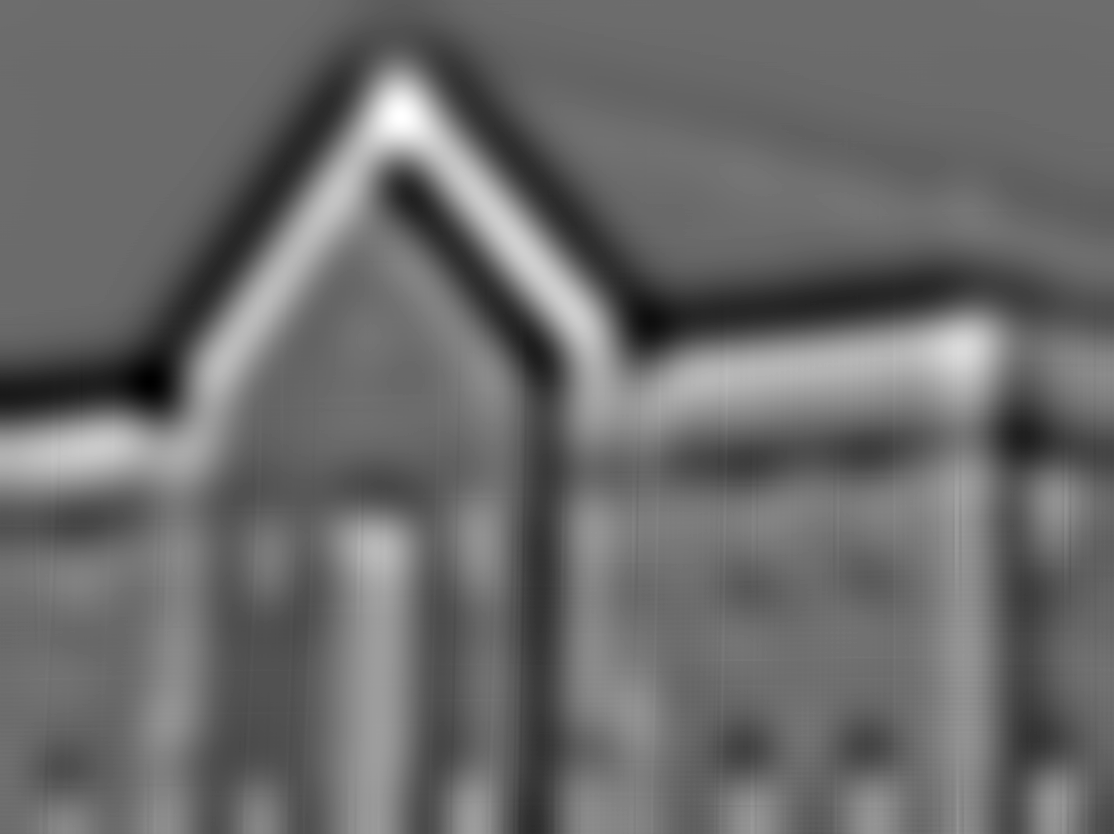
\includegraphics[height=60mm]{laplace201}
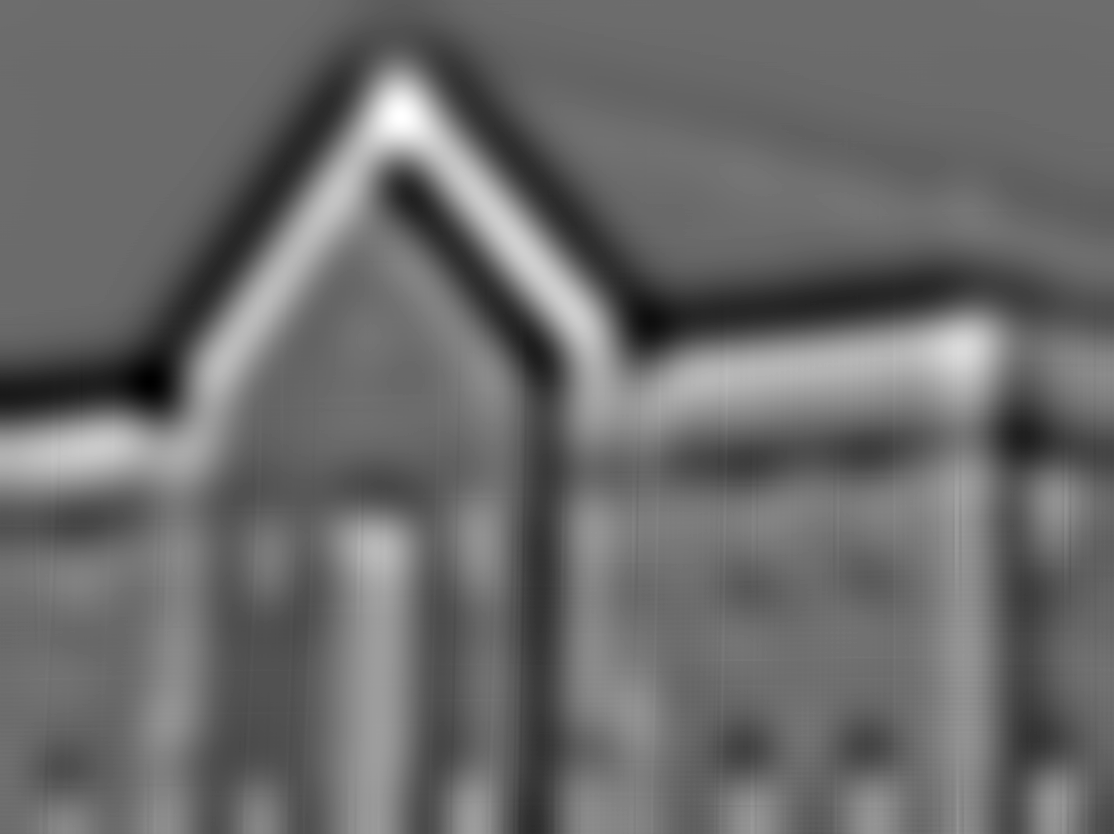
\includegraphics[height=60mm]{laplace301}
\newpage
House with zero crossing applied
\fbox{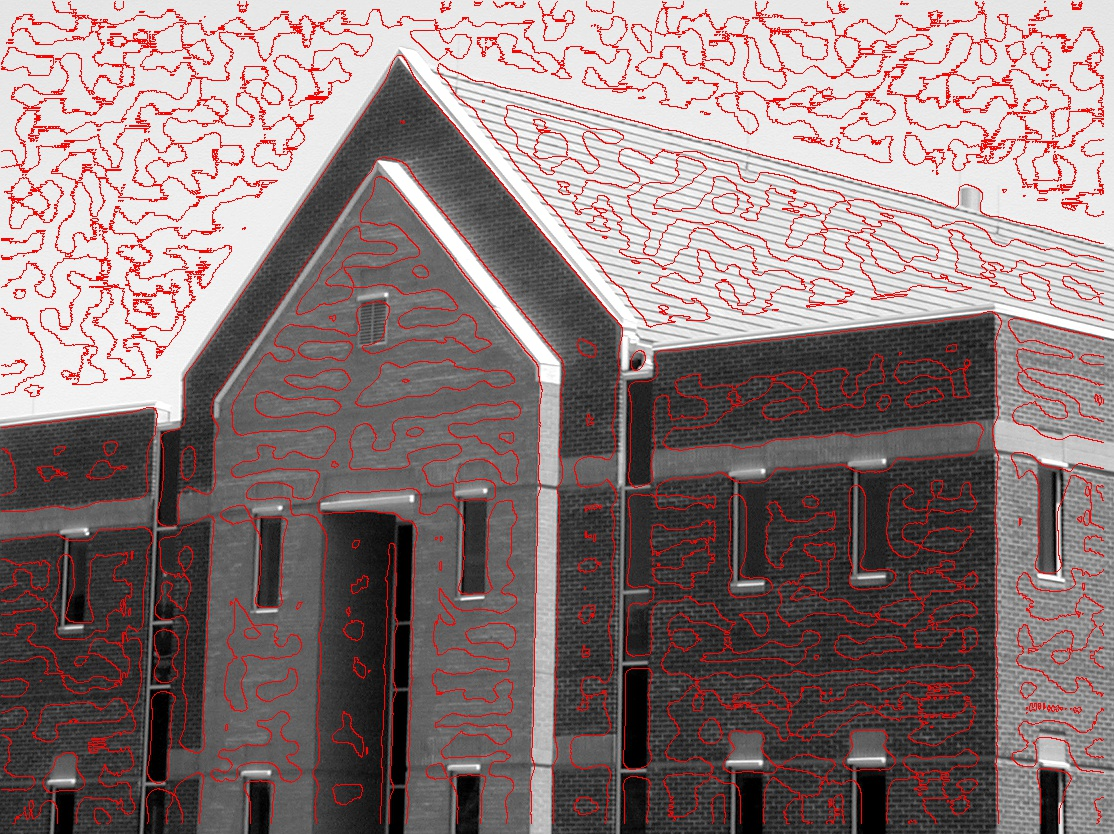
\includegraphics[height=60mm]{zerocross51}}
\fbox{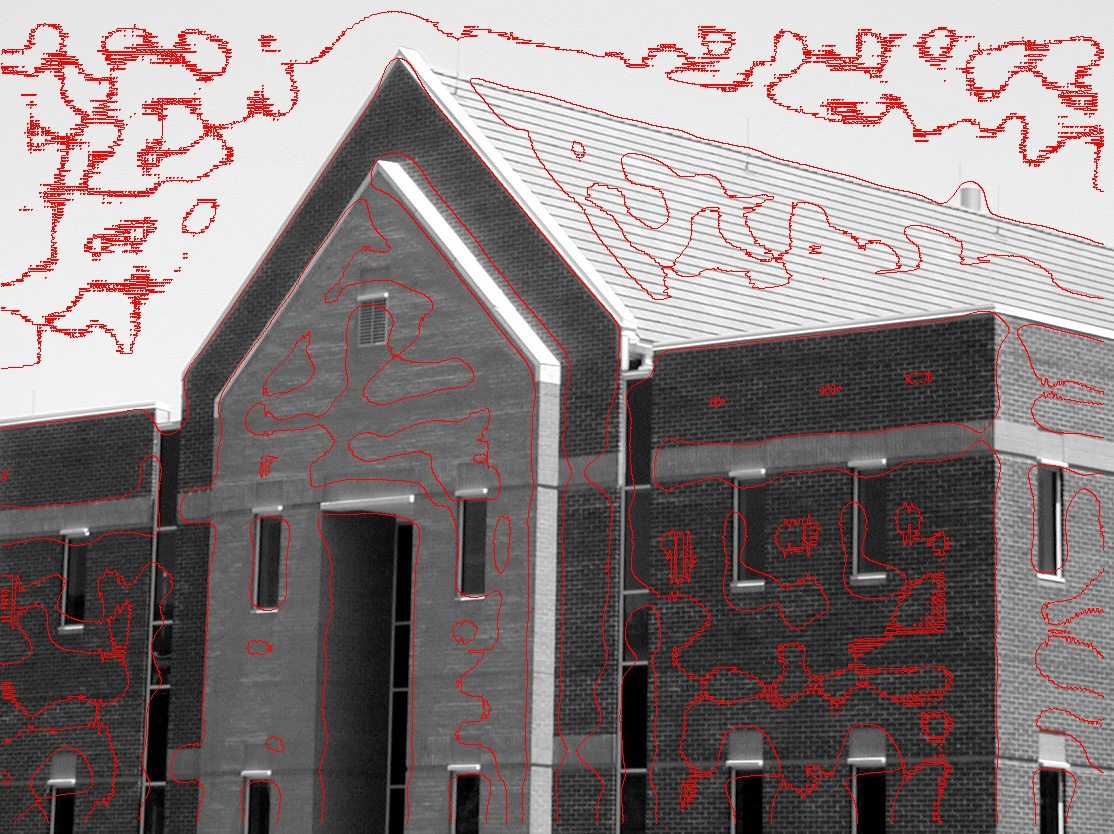
\includegraphics[height=60mm]{zerocross101}}
\fbox{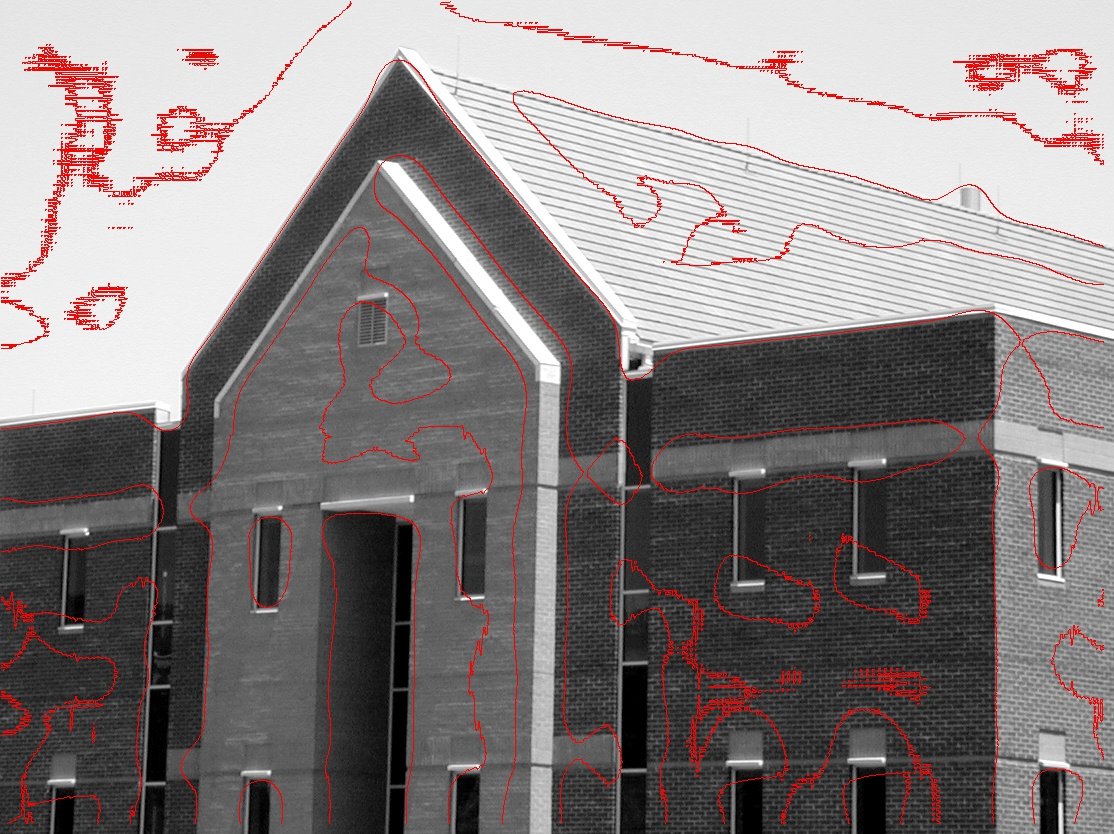
\includegraphics[height=60mm]{zerocross151}}
\fbox{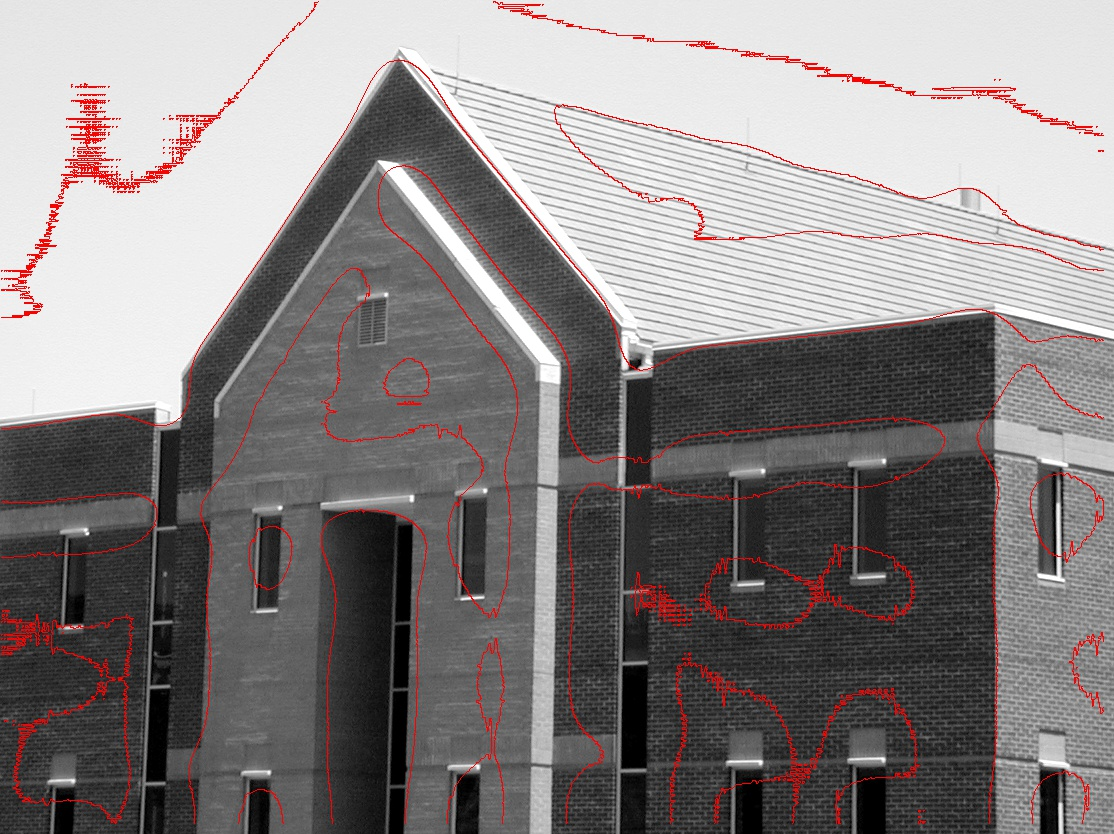
\includegraphics[height=60mm]{zerocross201}}
\fbox{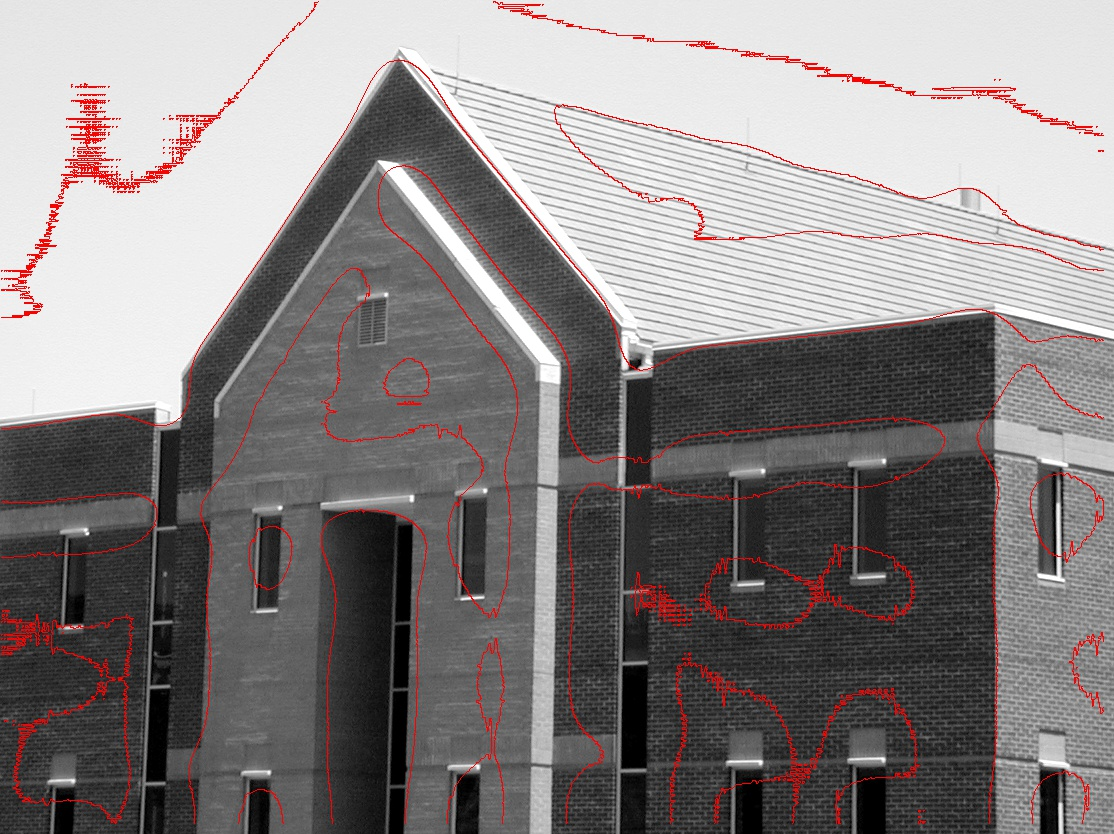
\includegraphics[height=60mm]{zerocross301}}

As the blurring was increased, the specificity of the zero crossing seemed to increases. With small amounts of blur, the zero crossing added red spots everywhere and with large amounts of blur the sprots are kind of the lines they should be.
\subsection{Time}
These took about 5 hours.
\newpage
\section{Homework}

\subsection{More strawberries}

\fbox{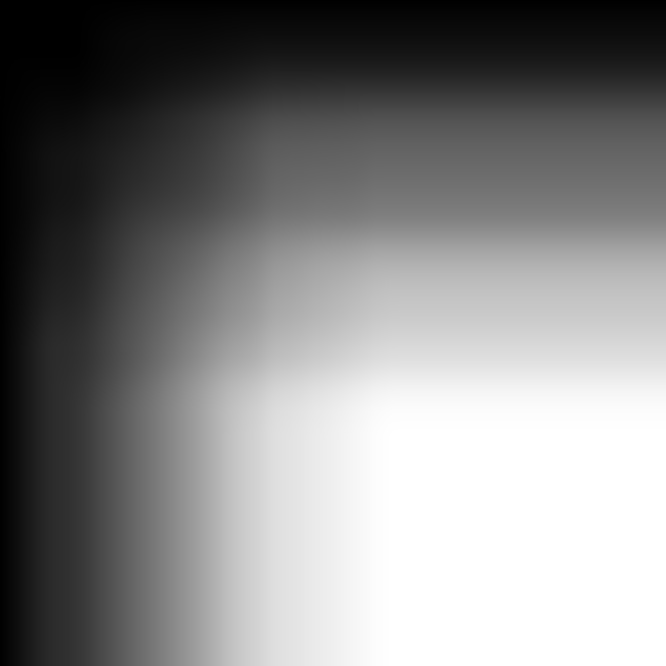
\includegraphics[height=120mm]{dpimage}}
Here is the heatmap for the integral image.

\fbox{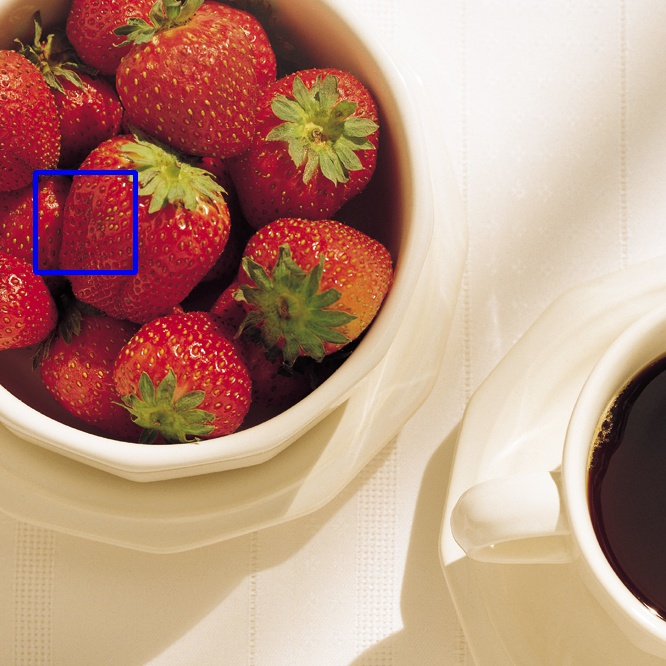
\includegraphics[height=120mm]{mostred}}
Here is the location that contained most red pixels. I found three zones that had the exact same count, but they were 1 pixel away from one another so there is only one square in the image.
\newpage
\subsection{Airports}
Here are some of the airport images with the Canny algorithm.
\fbox{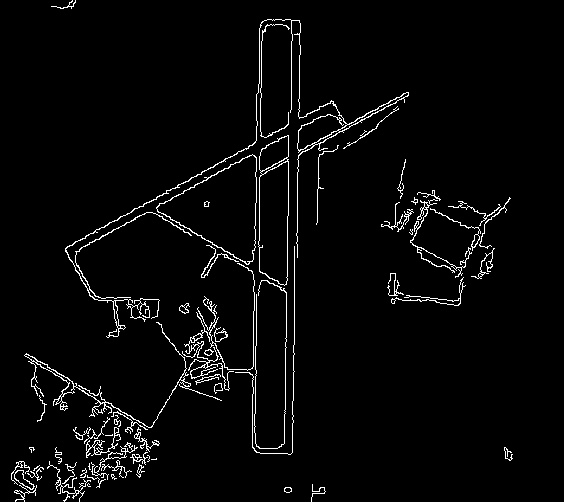
\includegraphics[height=50mm]{mairport175x575}}
\fbox{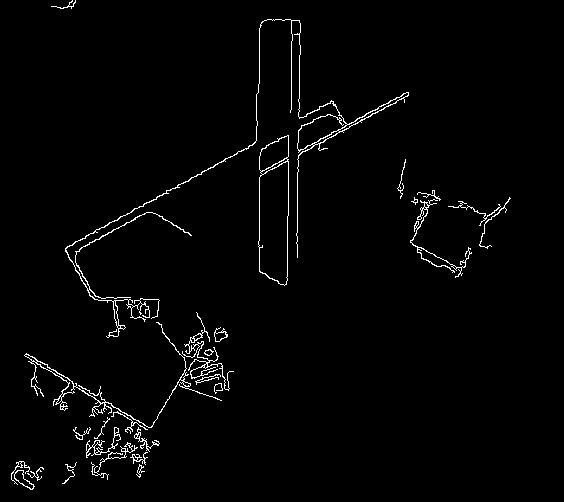
\includegraphics[height=50mm]{mairport175x700}}
\fbox{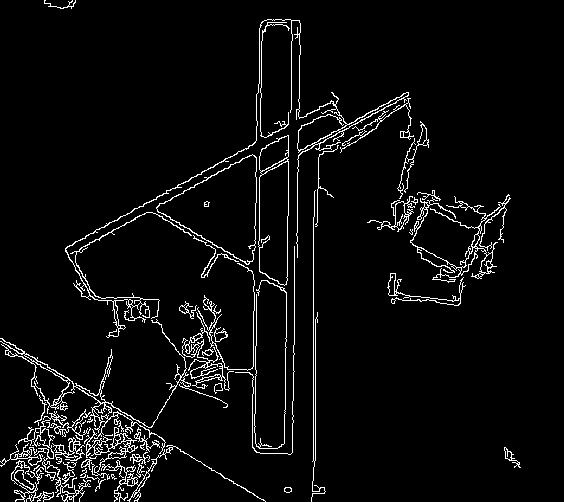
\includegraphics[height=50mm]{mairport100x575}}
\fbox{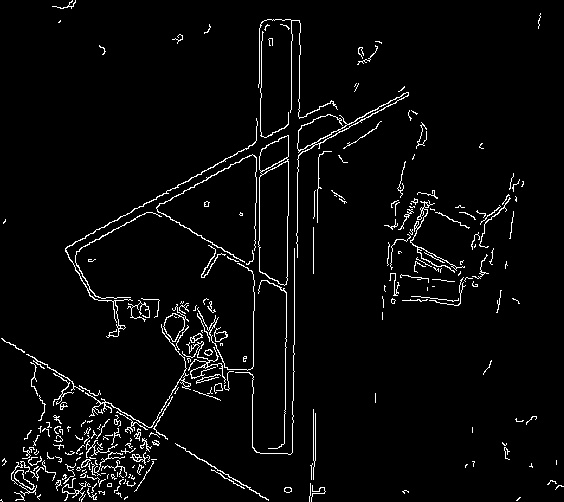
\includegraphics[height=50mm]{mairport225x400}}
\newpage
Here are Hough lines with 50, 80, 100 and 110.
\fbox{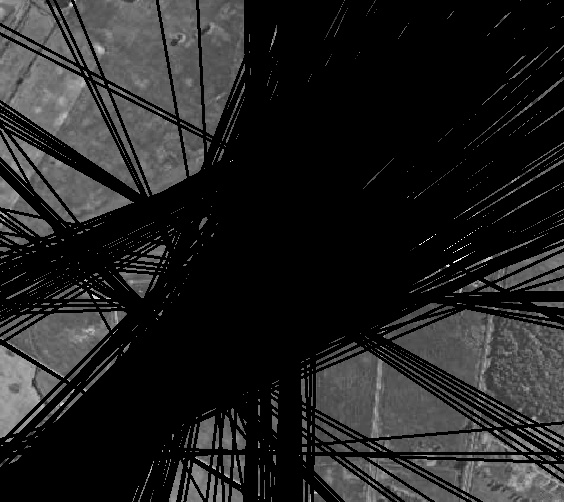
\includegraphics[height=50mm]{hmairport50}}
\fbox{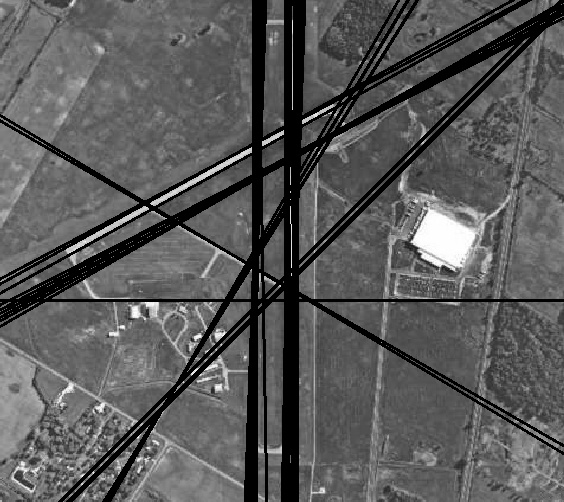
\includegraphics[height=50mm]{hmairport80}}
\fbox{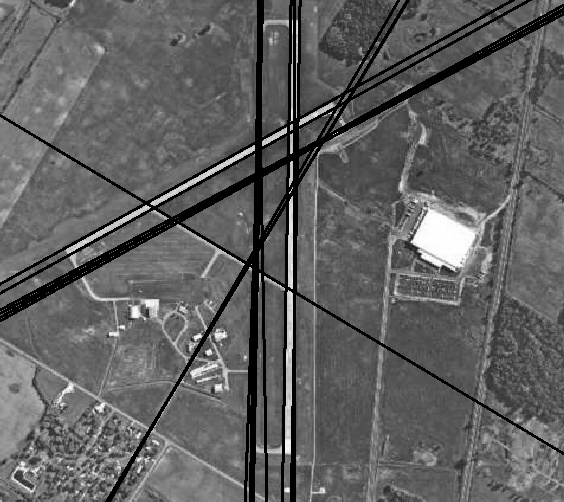
\includegraphics[height=50mm]{hmairport100}}
\fbox{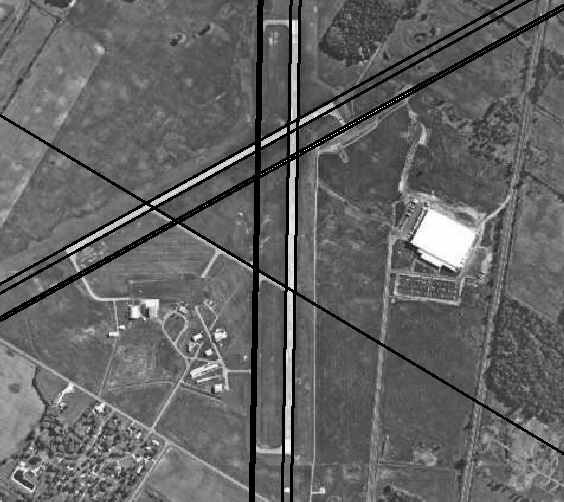
\includegraphics[height=50mm]{hmairport110}}
\pagebreak
\subsection{Parameters}
\begin{normalsize}


The Canny algorithm takes the image, a minimum value, maximum value and an optional aperture size parameter. The minimum value and maximum value specify regions where the edges are rejected or accepted. Between the values the edges are discarded or accepted depending on their continuity. The Hough Line transform takes an image, rho and theta values and a threshold. Here rho and theta are used in the function to determine the lines, and threshold is the amount of votes a line needs to be accepted.
\end{normalsize}
\subsection{Time}
This took about 5 hours
\newpage
\section{Code}

\begin{verbatim}
print('Reading images')

s = cv2.imread('strawberries-binary.pbm', cv2.IMREAD_GRAYSCALE)/255
strs = cv2.imread('strawberries.tiff')/255
b = cv2.imread('building.tiff', cv2.IMREAD_GRAYSCALE)/255
m = cv2.imread('marion_airport.tiff', cv2.IMREAD_GRAYSCALE)
print(b)
plt.imshow(m * 255)

def erode(A, k):
    return cv2.erode(s, k, iterations=1)


def dilate(A, k):
    return cv2.dilate(s, k, iterations=1)


def close(A, k):
    return cv2.morphologyEx(A, cv2.MORPH_CLOSE, k)


def open(A, k):
    return cv2.morphologyEx(A, cv2.MORPH_OPEN, k)

kernel3 = np.ones((3,3),np.uint8)
kernel1 = np.ones((1,1),np.uint8)
kernel5 = np.ones((5,5),np.uint8)
erosion = cv2.dilate(cv2.erode(s, kernel, iterations=1), kernel, iterations=1)
c = cv2.morphologyEx(s, cv2.MORPH_CLOSE, kernel)
closeopen = cv2.morphologyEx(c, cv2.MORPH_OPEN, kernel)
closeopendilate = cv2.dilate(closeopen, kernel, iterations=1)
# dilateclose = cv2.morphologyEx(dilate, cv2.MORPH_OPEN, kernel)
o = dilate(s, kernel3)
d = close(o, kernel3)
e = erode(s, kernel3)
# d = dilate(erode(e, kernel3), kernel3)
oppen = open(s, kernel3)

plt.imshow(oppen * 255)
cv2.imwrite('nopixelstrawberry.jpg',  oppen * 255)

def zerocrossing(A):
    (y, x) = A.shape
    newA = np.zeros([y, x, 3],dtype=np.float32)
    A = clip(np.pad(A, 1, 'edge'))
    for i in range(1, x - 10):
        for j in range(1, y - 10):
            val = A[(j, i)]
            lef = A[(j - 1, i)]
            top = A[(j, i - 1)]
            less = (val < 0) and (lef < 0) and (top < 0)
            greater = val > 0 and lef > 0 and top > 0
            zero = val == 0 and lef == 0 and top == 0
            if less or greater or zero:
                newA[(j, i )] = (0, 0, 0)
            else:
                newA[(j, i )] = (0, 0, 1)
    return newA
        
        
def blurit(A, i):
    return cv2.GaussianBlur(A,(i, i),0)

blr51 = blurit(b, 51)
blr101 = blurit(b, 101)
blr151 = blurit(b, 151)
blr201 = blurit(b, 201)
blr301 = blurit(b, 301)


# blr = blurit(blurit(blurit(blurit(blurit(b, 11), 51), 111), 151), 201)

cv2.imwrite('blurredhouse51.jpg',  blr51 * 255)
cv2.imwrite('blurredhouse101.jpg',  blr101 * 255)
cv2.imwrite('blurredhouse151.jpg',  blr151 * 255)
cv2.imwrite('blurredhouse201.jpg',  blr201 * 255)
cv2.imwrite('blurredhouse301.jpg',  blr301 * 255)
# for i in range(0, 9):
#     img = (cv2.GaussianBlur(img, (i*11,i*11), 0))

laplace51 = cv2.Laplacian(blr51, cv2.CV_64F)
plt.imsave("laplace51.jpg", clip(laplace51 + 0.5)*255, cmap=plt.cm.gray)
laplace101 = cv2.Laplacian(blr101, cv2.CV_64F)
plt.imsave("laplace101.jpg", clip(laplace101 + 0.5)*255, cmap=plt.cm.gray)
laplace151 = cv2.Laplacian(blr151, cv2.CV_64F)
plt.imsave("laplace151.jpg", clip(laplace151 + 0.5)*255, cmap=plt.cm.gray)
laplace201 = cv2.Laplacian(blr201, cv2.CV_64F)
plt.imsave("laplace201.jpg", clip(laplace201 + 0.5)*255, cmap=plt.cm.gray)
laplace301 = cv2.Laplacian(blr201, cv2.CV_64F)
plt.imsave("laplace301.jpg", clip(laplace201 + 0.5)*255, cmap=plt.cm.gray)
zerocross51 = (zerocrossing(laplace51))
zerocross101 = (zerocrossing(laplace101))
zerocross151 = (zerocrossing(laplace151))
zerocross201 = (zerocrossing(laplace201))
zerocross301 = (zerocrossing(laplace301))

for j in range(0, zerocross.shape[0]):
    for i in range(0, zerocross.shape[1]):
        (r, g, bl) = zerocross51[(j, i)]
        if r == 0 and g == 0 and bl == 0:
            zerocross51[j][i] = b[j][i]
            
for j in range(0, zerocross.shape[0]):
    for i in range(0, zerocross.shape[1]):
        (r, g, bl) = zerocross101[(j, i)]
        if r == 0 and g == 0 and bl == 0:
            zerocross101[j][i] = b[j][i]
            
for j in range(0, zerocross.shape[0]):
    for i in range(0, zerocross151.shape[1]):
        (r, g, bl) = zerocross151[(j, i)]
        if r == 0 and g == 0 and bl == 0:
            zerocross151[j][i] = b[j][i]
            
for j in range(0, zerocross.shape[0]):
    for i in range(0, zerocross.shape[1]):
        (r, g, bl) = zerocross201[(j, i)]
        if r == 0 and g == 0 and bl == 0:
            zerocross201[j][i] = b[j][i]
            
for j in range(0, zerocross.shape[0]):
    for i in range(0, zerocross.shape[1]):
        (r, g, bl) = zerocross301[(j, i)]
        if r == 0 and g == 0 and bl == 0:
            zerocross301[j][i] = b[j][i]
    
plt.imshow(clip(laplace) * 255)
cv2.imwrite('zerocross51.jpg',  zerocross51 * 255)
cv2.imwrite('zerocross101.jpg',  zerocross101 * 255)
cv2.imwrite('zerocross151.jpg',  zerocross151 * 255)
cv2.imwrite('zerocross201.jpg',  zerocross201 * 255)
cv2.imwrite('zerocross301.jpg',  zerocross301 * 255)

# cv2.imwrite('zc.jpg',  laplace * 255)

print(s.shape)
(v, ss) = cv2.threshold(s,0.5,1,cv2.THRESH_BINARY)
npss = np.array(ss)
print (npss)
def iifs(img):
    (w, h) = img.shape
    dp = np.zeros([w, h], dtype=np.int64)
    A = img
    for i in (range(w)):
        for j in range(h):
            if i == 0 and j == 0:
                dp[i][j] = A[i][j]
            elif i == 0:
                dp[i][j] = dp[i][j-1] + A[i][j]
            elif j == 0:
                dp[i][j] = dp[i-1][j] + A[i][j]
            else:
                dp[i][j] = dp[i-1][j] + A[i][j] + (dp[i][j - 1] - dp[i-1][j-1])
                
    return dp

ifsres = iifs(npss)
plt.imshow((ifsres / np.max(ifsres)) * 255)

cv2.imwrite('dpimage.jpg',  255*(ifsres / np.max(ifsres)))

def iif(dp):
    (w, h) = dp.shape
    maxv = 0
    maxc = (0, 0)
    for i in range(1, (w - 101)):
        for j in range(1, (h - 101)):
            br = dp[i + 99][j + 99]
            bl = dp[i + 99][j - 1]
            tr = dp[i - 1][j + 99]
            tl = dp[i - 1][j - 1]
            tot = br - bl - tr + tl
            if tot > 0:
                if tot > maxv:
                  maxv = tot
                  maxc = (i, j)
                if tot == maxv:
                  print(maxv, i, j)
            
    return (maxv, maxc)
bestarea = iif(ifsres)
print (bestarea)

square = cv2.rectangle(strs, (35, 172), (135, 272), (1, 0, 0), 4)

plt.imshow(square)

cv2.imwrite('mostred.jpg',  255*square)


edges = cv2.Canny(m,570, 200, apertureSize = 3)

plt.imshow(edges)
cv2.imwrite('mairport.jpg', edges)
cv2.imwrite('mairport175x575.jpg', cv2.Canny(m,175,575))
cv2.imwrite('mairport175x700.jpg', cv2.Canny(m,175,700))
cv2.imwrite('mairport100x575.jpg', cv2.Canny(m,100,575))
cv2.imwrite('mairport225x400.jpg', cv2.Canny(m,225,400))

e = edges
img = np.array(m, copy=True)
lines = cv2.HoughLines(e, 1,np.pi/180,110)
for l in lines:
    (rho,theta) = l[0]
    a = np.cos(theta)
    b = np.sin(theta)
    x0 = a*rho
    y0 = b*rho
    x1 = int(x0 + 1000*(-b))
    y1 = int(y0 + 1000*(a))
    x2 = int(x0 - 1000*(-b))
    y2 = int(y0 - 1000*(a))
    cv2.line(img,(x1,y1),(x2,y2),(0,0,255),2)
plt.imshow(img)
cv2.imwrite('hmairport110.jpg', img)
\end{verbatim}
\subsection{Pre and post normalization histograms}

\end{document}
